\documentclass[20pt,a4paper,landscape]{extarticle}
\usepackage[margin=1.45cm,top=0.45cm,left=0.9cm,right=0.9cm,bottom=0.9cm]{geometry}
\usepackage{amsmath}
\usepackage{amssymb}
\usepackage{graphicx}
\usepackage{xcolor}
\usepackage[sfdefault,lf]{FiraSans}
\renewcommand{\familydefault}{\sfdefault}
\setlength{\parindent}{0pt}
\pagestyle{empty}
\everymath{\displaystyle}
\begin{document}
\sffamily
\boldmath
{\LARGE \textbf{Estimating lengths from scale drawings and photos --- Foundation}}\par\vspace{0.45em}
\begin{center}
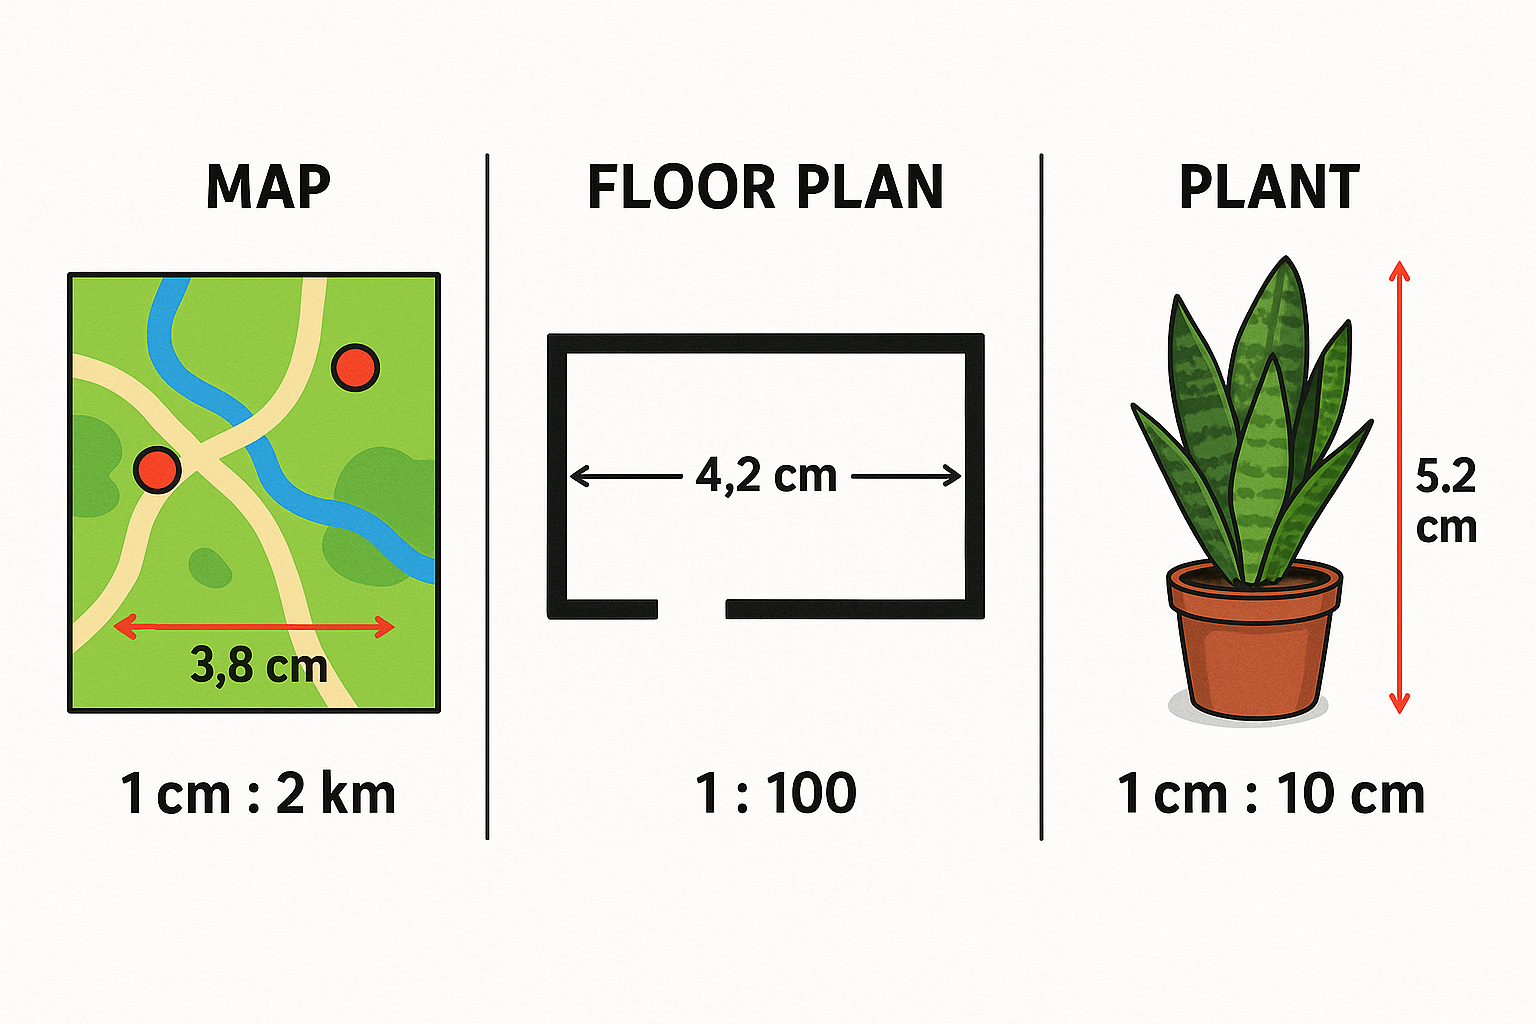
\includegraphics[width=0.94\linewidth,height=0.49\textheight,keepaspectratio]{web-diagrams/foundation-composite.png}
\end{center}
\vspace{0.35em}
\noindent\begin{minipage}[t]{0.275\linewidth}\vspace{0pt}\textbf{1.} Use the map to estimate the real distance between the two marked points.\end{minipage}\hspace{0.08\linewidth}\begin{minipage}[t]{0.275\linewidth}\vspace{0pt}\textbf{2.} Use the floor plan to estimate the real room length in metres.\end{minipage}\hspace{0.08\linewidth}\begin{minipage}[t]{0.275\linewidth}\vspace{0pt}\textbf{3.} Use the plant measurements to estimate the real plant height in cm.\end{minipage}\par

\vspace{1.0em}
\begin{center}
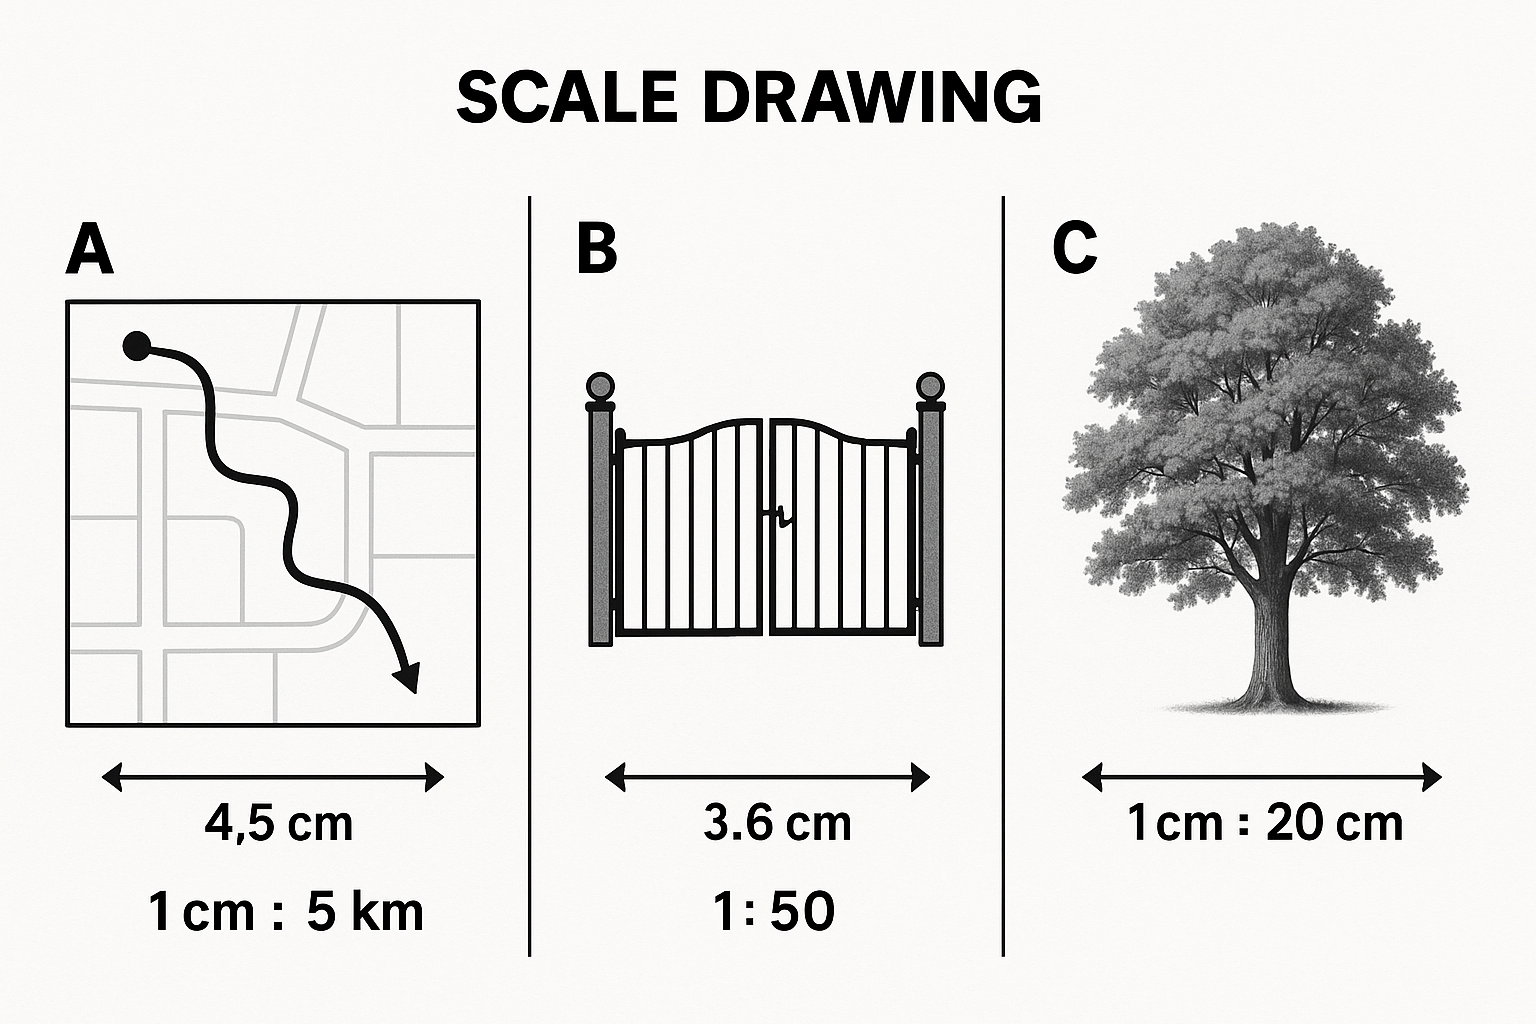
\includegraphics[width=0.94\linewidth,height=0.49\textheight,keepaspectratio]{web-diagrams/foundation-composite-2.png}
\end{center}
\vspace{0.35em}
\noindent\begin{minipage}[t]{0.275\linewidth}\vspace{0pt}\textbf{4.} Use the route map to estimate the real distance shown.\end{minipage}\hspace{0.08\linewidth}\begin{minipage}[t]{0.275\linewidth}\vspace{0pt}\textbf{5.} Use the gate drawing to estimate the real gate width in cm.\end{minipage}\hspace{0.08\linewidth}\begin{minipage}[t]{0.275\linewidth}\vspace{0pt}\textbf{6.} Use the tree measurements to estimate the real tree height.\end{minipage}\par

\vspace{1.0em}
\noindent\begin{minipage}[t]{0.46\linewidth}\vspace{0pt}\textbf{7.} A map scale is $1$ cm : $3$ km. A path measures $2.5$ cm on the map. Estimate the real distance.\end{minipage}\hfill\begin{minipage}[t]{0.46\linewidth}\vspace{0pt}\textbf{8.} A photo scale is $1$ cm : $8$ cm. A fish is $4.5$ cm long in the photo. Estimate the real fish length.\end{minipage}
\end{document}
